\documentclass[11pt,a4paper,twocolumn]{amsart}

\usepackage[
  a4paper,
  top=13mm,
  bottom=15mm,
  left=12mm,
  right=12mm
]{geometry}
\setlength{\columnsep}{4mm}
\usepackage[utf8]{inputenc}
\usepackage[T1]{fontenc}
\usepackage{newtxtext,newtxmath}
\usepackage{microtype}
\emergencystretch=3em
\clubpenalty=10000
\widowpenalty=10000
\displaywidowpenalty=10000
\brokenpenalty=10000
\hyphenation{exemplar Monterey}
\usepackage{mathtools}
\usepackage{graphicx}
\usepackage{caption}
\captionsetup{
  style=base,
  format=plain,
  margin=0pt,
  width=\linewidth,
  font=footnotesize,
  labelfont=bf,
  labelsep=period,
  justification=raggedright,
  singlelinecheck=false,
  skip=4pt
}
\renewcommand{\figurename}{Figure}
\setlength{\captionindent}{0pt}
\usepackage{xcolor}
\usepackage{tikz}
\usepackage{hyperref}
\usepackage{xurl}

\hypersetup{
  colorlinks=true,
  linkcolor=black,
  citecolor=black,
  urlcolor=blue
}

\title{Software Engineering for AI/AS and Multi-Vehicle Maritime Robotics}
\author{Shekhar Devm Upadhyay}
\address{KTH Royal Institute of Technology / SMaRC / WASP}
\date{September 2026}

\begin{document}
\maketitle

\begin{figure}[t]
\centering
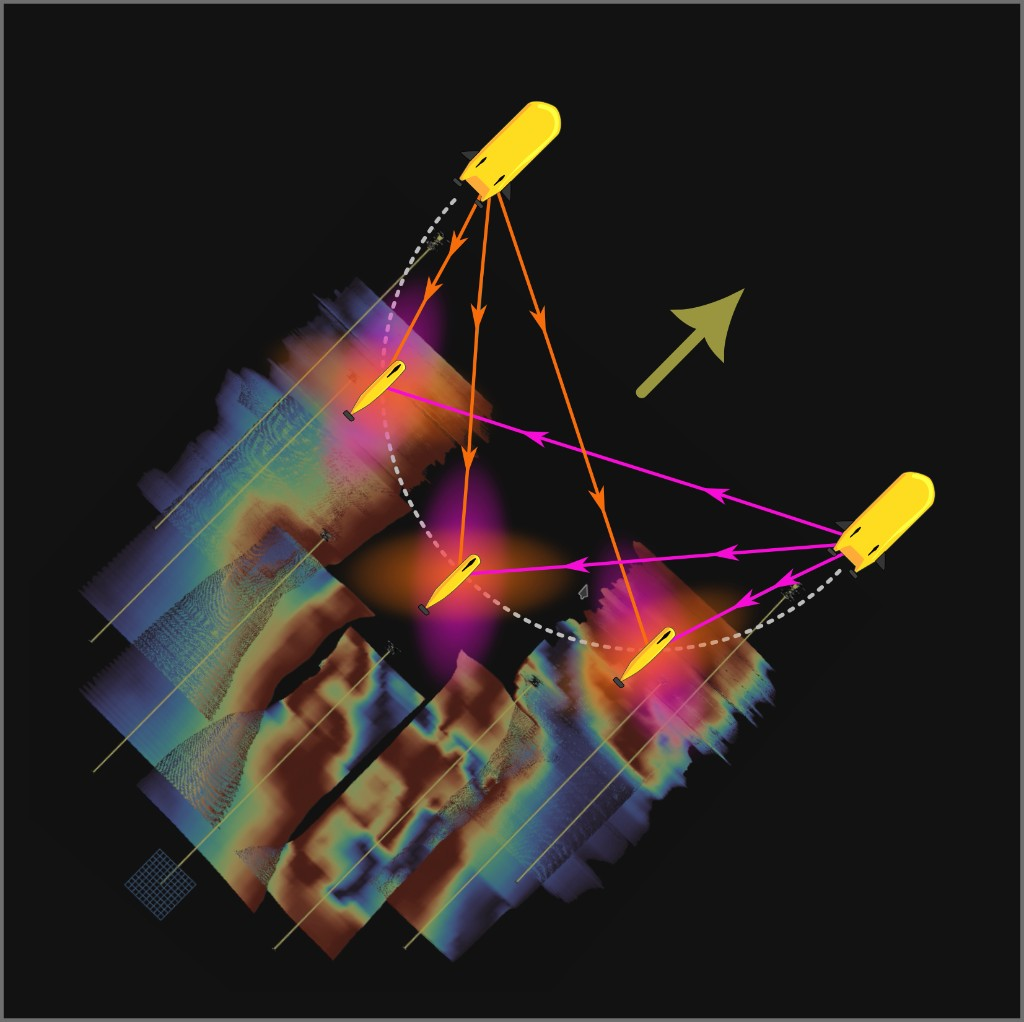
\includegraphics[width=\columnwidth]{figures/tuper_fleet.jpg}
\caption{Illustration of the intended TUPER fleet on a bathymetric prior: leaders range to followers; overlapping sidescan swaths \mbox{are the map product.}}
\label{fig:fleet}
\end{figure}

\section{Introduction}
\label{sec:intro}

I am a WASP PhD student at the Swedish Maritime Robotics Centre (SMaRC) at KTH, supervised by John Folkesson. The project is TUPER (Team Underwater Perception for Event Response), connected to WARA-PS (WASP Research Arena for Public Safety). European coastal waters now hold cables, pipelines, wind farms, and aquaculture. A ruptured pipeline or wreck needs a map of a large area. Large autonomous underwater vehicles (AUVs) are slow to launch. The team is mostly smaller, hand-deployable vehicles, led by one or two with good navigation. High-resolution mapping needs the team close to the seabed, which shrinks each swath, so several vehicles run in a fixed formation. Simple sensors georeference poorly. The intended ranging method is synchronized one-way travel time (OWTT), \mbox{fused with onboard navigation.}

OWTT needs agreeing clocks. A surface leader with a Global Navigation Satellite System (GNSS) receiver broadcasts a timestamped position; range is travel time times sound speed. We published the formation and localization work at IEEE OCEANS 2025 (Great Lakes). That trial had no shared clock, so the protocol was two-way travel time (TWTT). Figure~\ref{fig:drone} is that trial from the air: two WARA-PS mini uncrewed surface vehicles (USVs) as leaders and LoLo, the KTH AUV, as the follower.

\begin{figure}[t]
\centering
\begin{tikzpicture}
\node[anchor=south west,inner sep=0] (image) at (0,0) {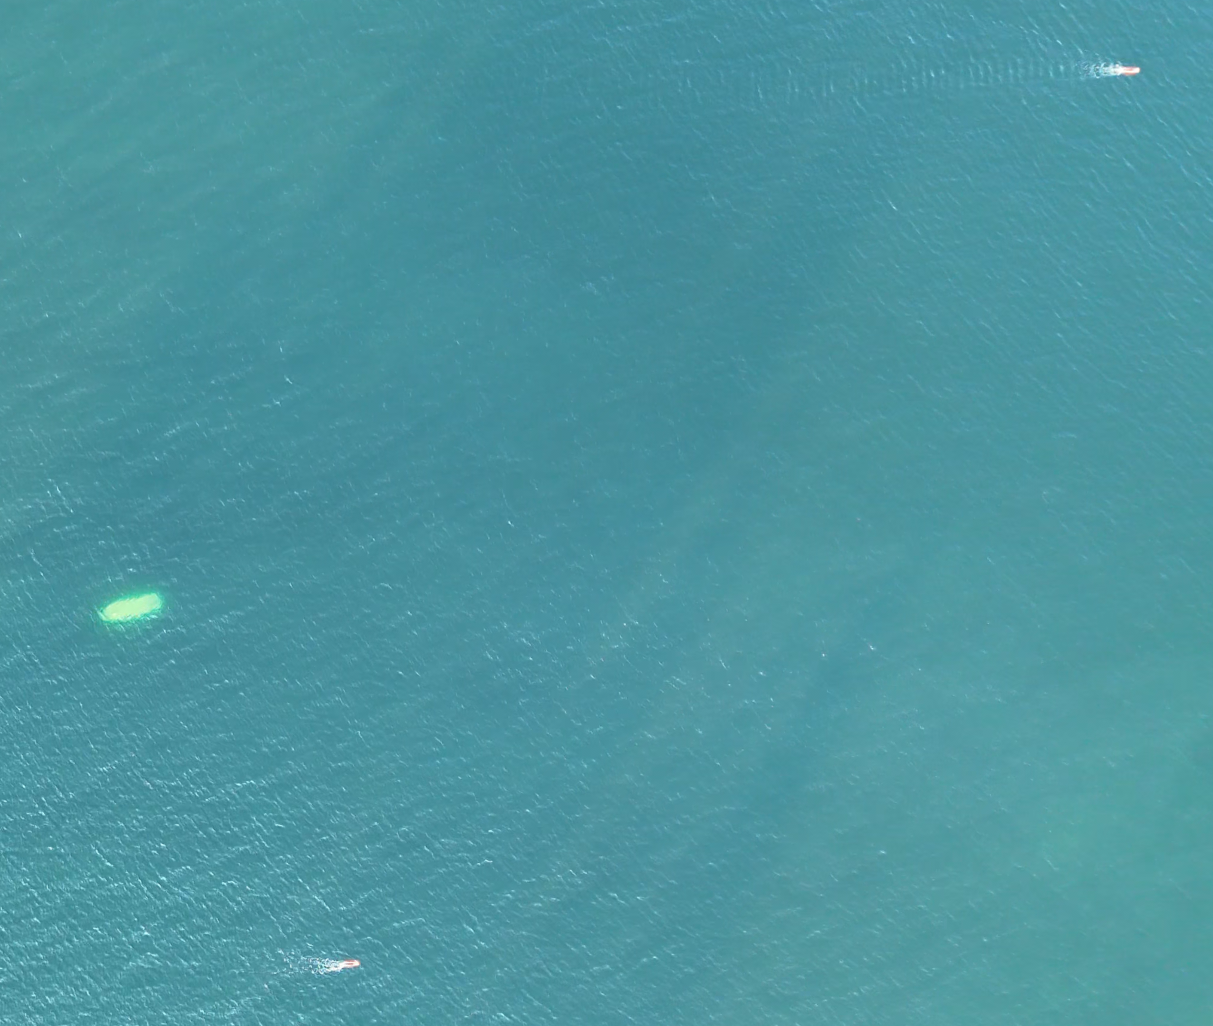
\includegraphics[width=\columnwidth]{figures/drone_asko.png}};
\begin{scope}[x={(image.south east)},y={(image.north west)}]
\node[fill={rgb,255:red,255;green,127;blue,14}, text=white, rounded corners=2pt, font=\scriptsize\bfseries]
      at (0.84, 0.85) {Leader 1};
\node[fill={rgb,255:red,148;green,103;blue,189}, text=white, rounded corners=2pt, font=\scriptsize\bfseries]
      at (0.30, 0.15) {Leader 2};
\node[fill=blue!70, text=white, rounded corners=2pt, font=\scriptsize\bfseries]
      at (0.15, 0.30) {Follower (LoLo)};
\end{scope}
\end{tikzpicture}
\caption{Aerial photograph of the 2025 ranging trial at Ask\"{o}: two WARA-PS mini-USVs as surface leaders and \mbox{LoLo as the follower.}}
\label{fig:drone}
\end{figure}

We timestamp those same modems against GNSS pulse-per-second (PPS) at the surface and an oven-controlled oscillator (OCXO) in holdover. That clock-and-ranging method is accepted at IEEE OCEANS 2026 (Monterey). On ice, one-way ranging still returns a range at $621.86$~m where two-way times out. In harbour water, clear paths match concurrent real-time kinematic (RTK) GNSS at decimetre root-mean-square error (RMSE). Uncorrected holdover on the three-hour pier moor is $-48.1$ parts per billion (ppb), or $-0.256$~m/h. After one hour of PPS, 48~h of free-run accumulates $10.8$~cm (Figure~\ref{fig:holdover}).

\begin{figure}[t]
\centering
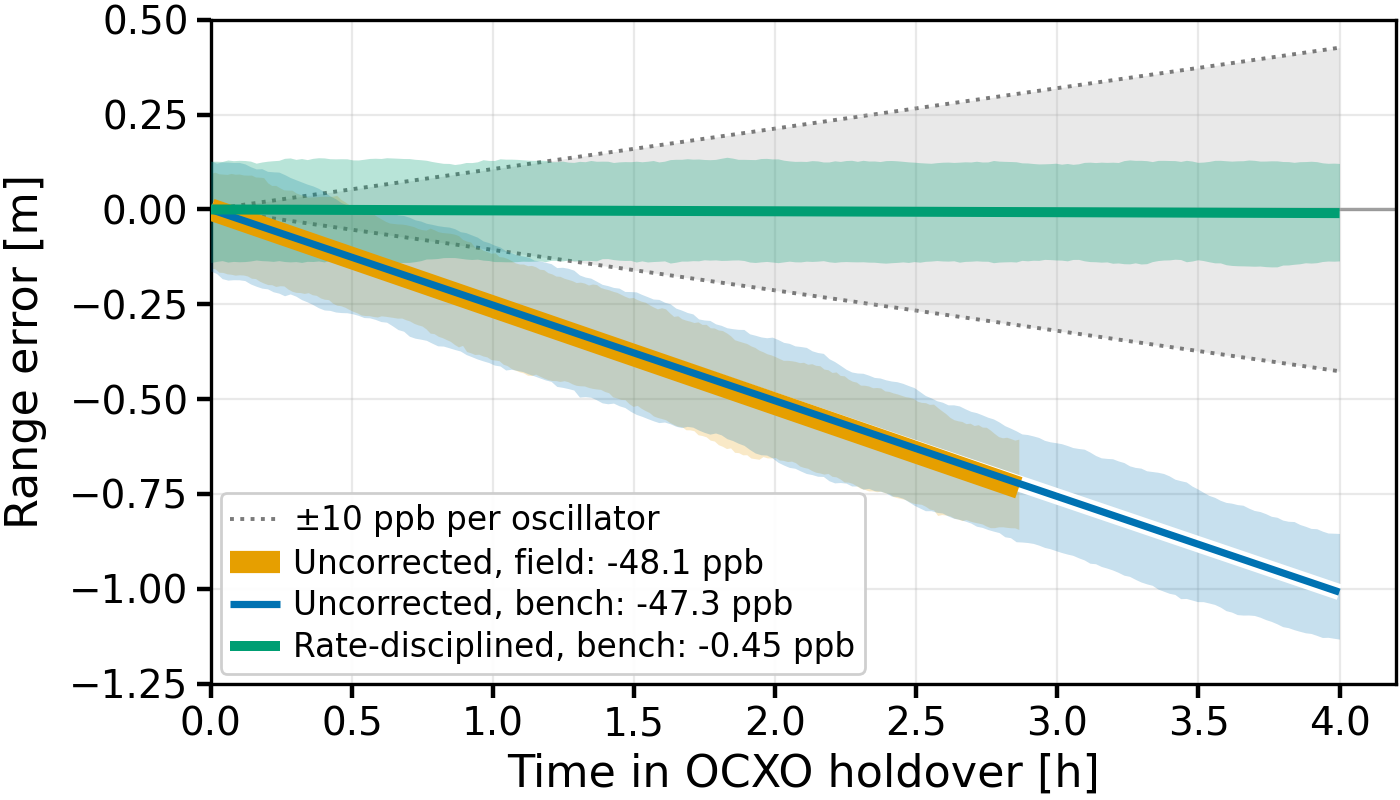
\includegraphics[width=\columnwidth]{figures/ocxo_holdover.png}
\caption{OCXO holdover after the last PPS lock: \mbox{uncorrected and rate-disciplined traces.}}
\label{fig:holdover}
\end{figure}

The team stays in formation through ranging. Mapping still needs a tighter trajectory. At a later Ask\"{o} survey, from a pole-mounted vessel, we registered 3D sidescan (3DSS) clouds to a prior bathymetric map with Generalized Iterative Closest Point (GICP) and added those alignments as factors next to dead-reckoning odometry in a factor graph. We published that trajectory-correction method at the IEEE/OES Autonomous Underwater Vehicles Symposium in 2026. GNSS and an inertial navigation system (INS) on the vessel were the reference. At synthetic $1\%$ of distance travelled on the $1197$~m track, 2D RMSE fell from $10.46$~m to \mbox{$1.62$~m (Figure~\ref{fig:asko-map}).}

\begin{figure}[t]
\centering
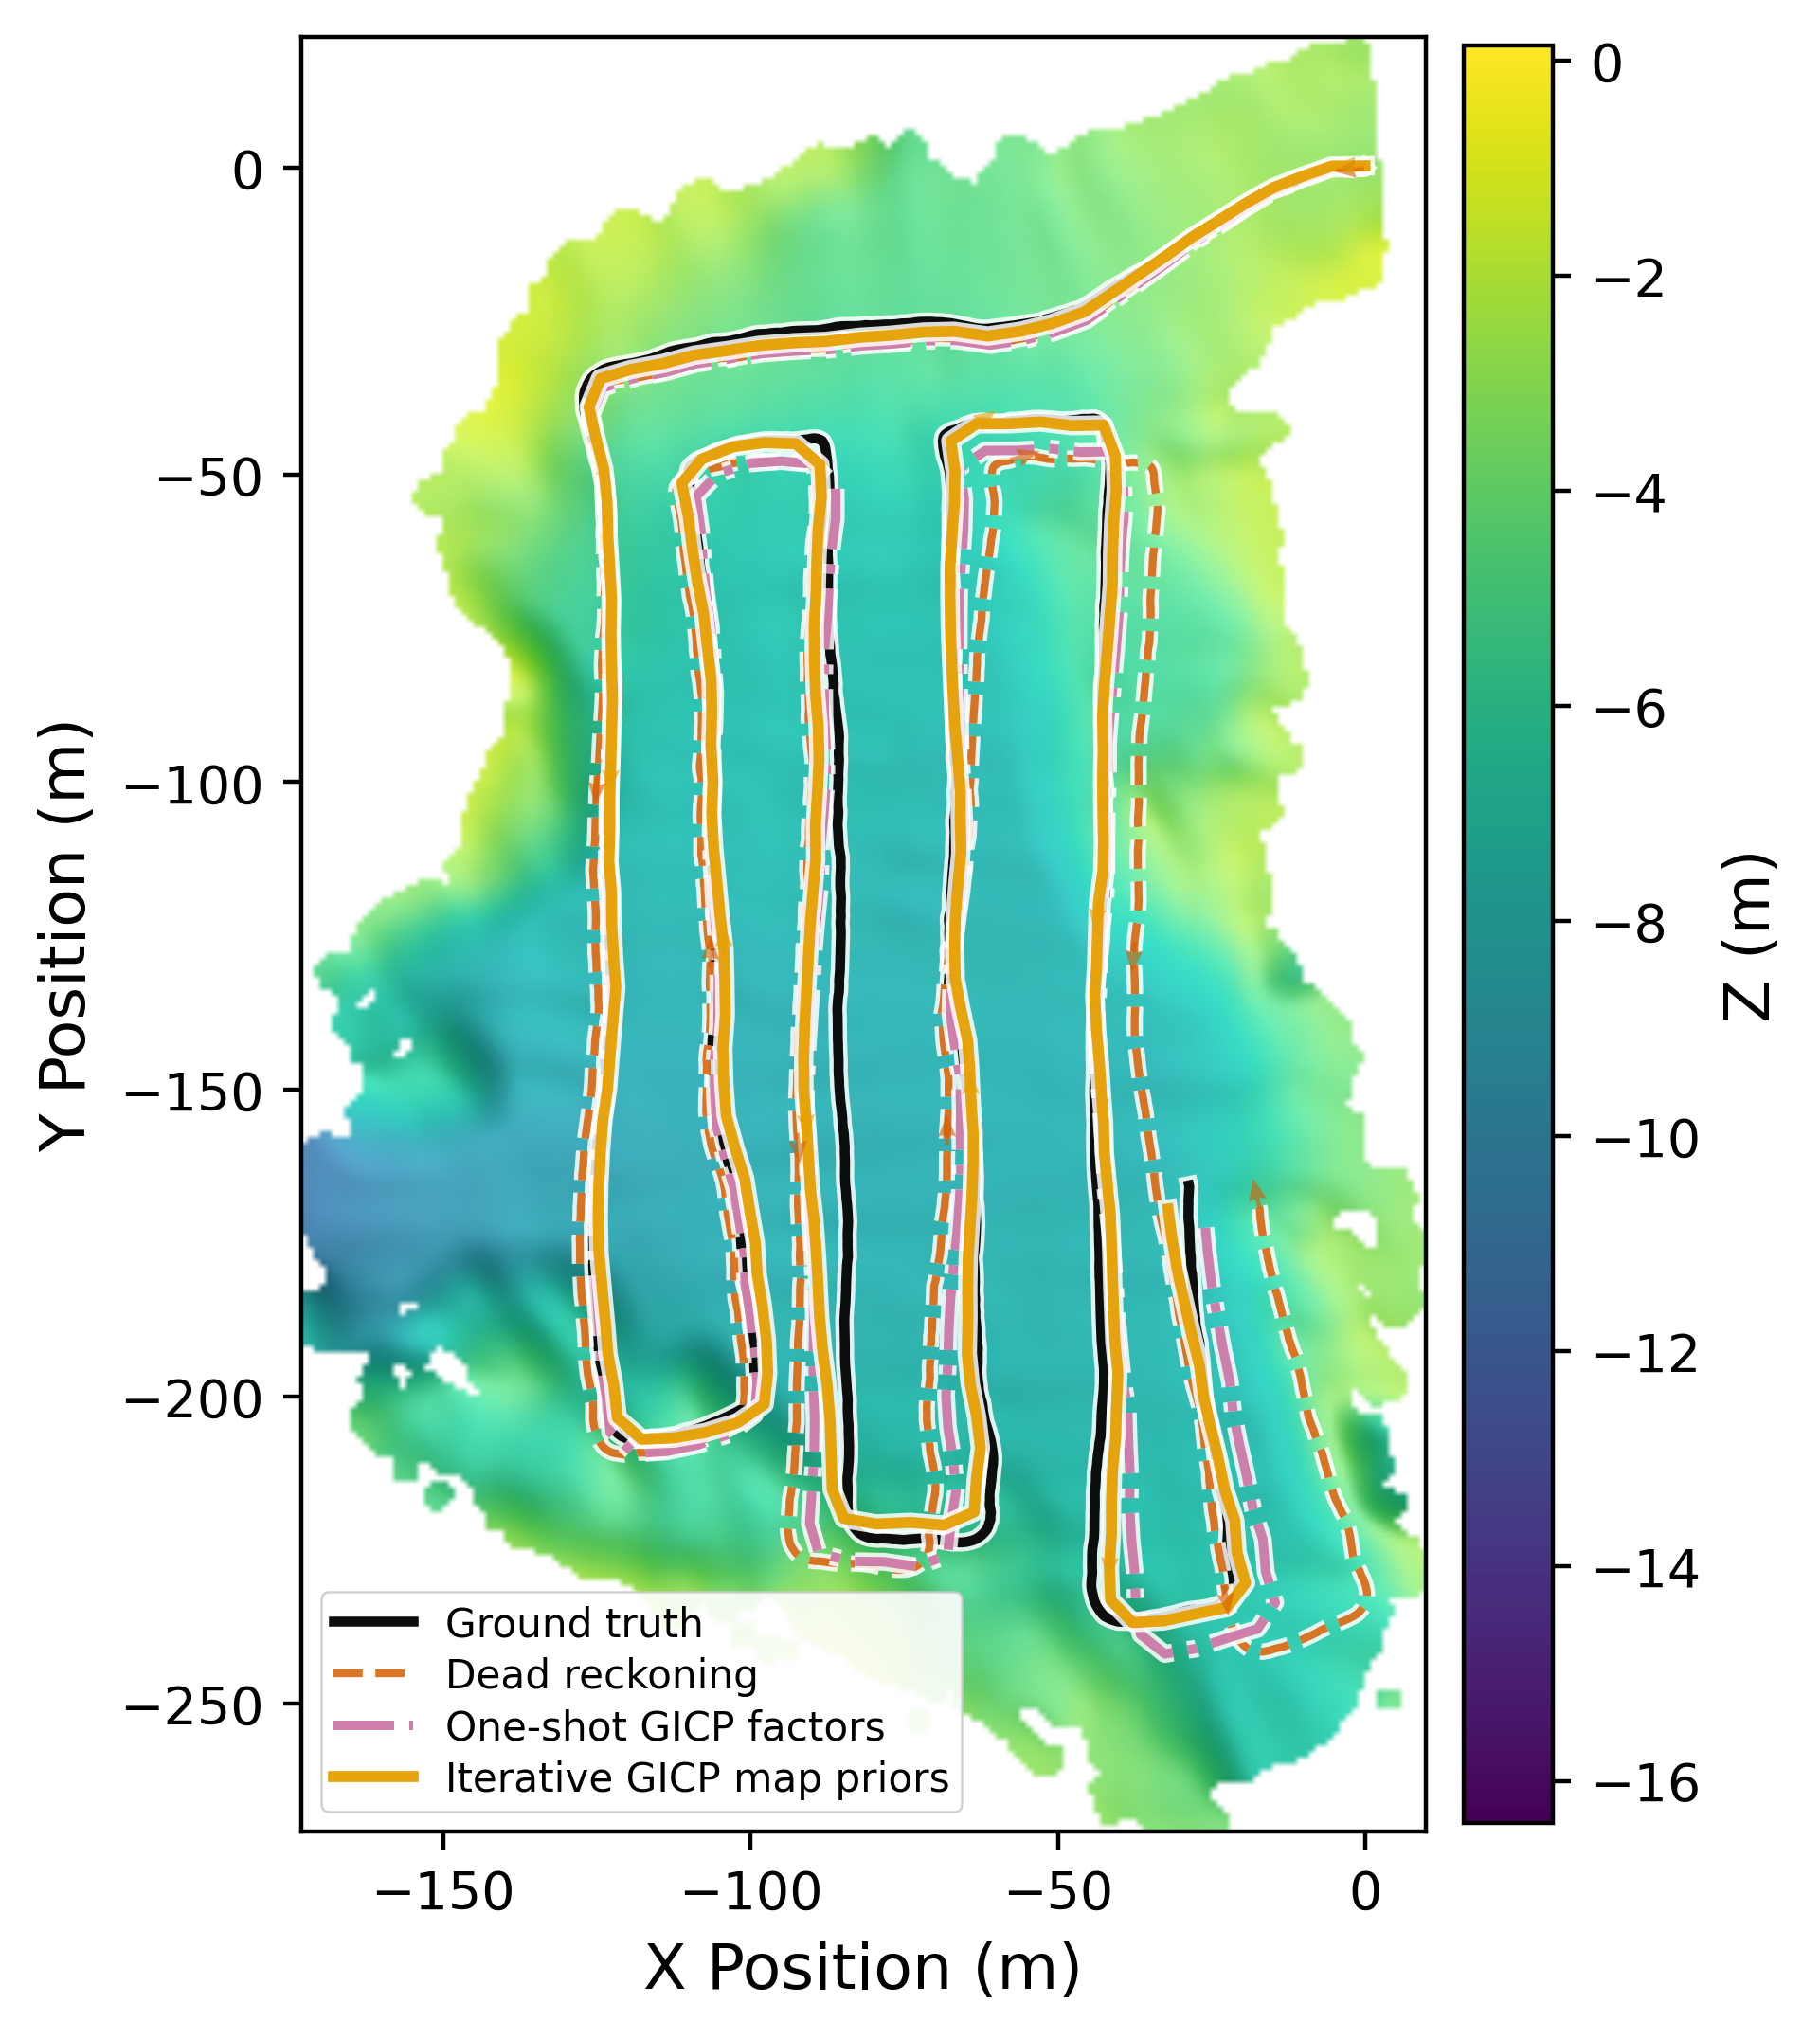
\includegraphics[width=\columnwidth]{figures/paper_trajectory_overlay_hillshade_broad.png}
\caption{Later Ask\"{o} 3D-sidescan survey from a pole-mounted vessel: dead-reckoned and GICP-optimized trajectories at \mbox{synthetic $1\%$ of distance travelled.}}
\label{fig:asko-map}
\end{figure}

The 3DSS was in that survey because it already emits 3D points, so we could show the backend. The TUPER fleet will mostly carry conventional 2D sidescan. If we lift those 2D images toward 3DSS-like geometry, the same scan-to-map backend can run on every hull. Scan-to-scan between vehicles is the extra fleet step. The product is a team that launches, covers the scene, and returns with a consistent map; this essay treats that product as the AI Engineering~problem.

\section{Lecture principles}
\label{sec:lecture}

\subsection{Hidden technical debt, and testing as validation}
\label{sec:debt}

Robert's L01 discussion of Sculley et al.\ names two recurring costs in ML-style systems. Glue is the wrapper that connects a model or estimator to the rest of the stack. Undeclared data dependencies are inputs the pipeline uses without listing them, so a replay six months later silently disagrees. In a field-robotics stack those costs look like this. Every node that talks to the acoustic modem opens the serial port itself, so you cannot swap the hardware or replay a trial without touching the estimator. Topic names and ranging dialects live in someone's head, so last year's recorded trial will not play through this year's nodes. The design idea is to split those layers: one package owns the physical device; other packages own protocols, missions, and tests; READMEs say which experiment a launch belongs to.

The acoustic stack (\href{https://github.com/NinjaTuna007/serial_ping_pkg}{\texttt{serial\_ping\_pkg}}) is public. Ranging and relay nodes live in one Robot Operating System 2 (ROS~2) package. The serial driver is a \emph{separate} ROS~2 package (\href{https://github.com/NinjaTuna007/succorfish_driver}{\texttt{succorfish\_driver}}), pulled in as a submodule. A single driver node opens the port and republishes raw lines and bytes; leader and follower nodes only subscribe. Three reasons: two processes cannot share a serial port; the ranging logic can run against a fake driver in pytest, with no modem on the desk; USB modem versus Teensy clock front-end is selected in the launch file. Topic names sit in a message definition (\href{https://github.com/NinjaTuna007/succorfish_driver/blob/main/succorfish_msgs/msg/Topics.msg}{\texttt{Topics.msg}}), not as string literals in nodes. Each experimental dialect has its own code, YAML, launch, tests, and README: \href{https://github.com/NinjaTuna007/serial_ping_pkg/blob/main/serial_ping_pkg/serial_ping_pkg/tuper_twtt/README.md}{two-way ranging} versus \href{https://github.com/NinjaTuna007/serial_ping_pkg/blob/main/serial_ping_pkg/serial_ping_pkg/tuper_owtt/README.md}{one-way ranging}. The \href{https://github.com/NinjaTuna007/serial_ping_pkg/blob/main/serial_ping_pkg/README.md}{package README} says which launch to run and that the two ranging dialects are different trees. SMaRC's shared vehicle software, \href{https://github.com/smarc-project/smarc2}{\texttt{smarc2}}, does the same at centre scale: the \href{https://github.com/smarc-project/smarc2/blob/humble/README.md}{root README} says where behaviours live and when a package should be a submodule.

The debt we actually pay is backward compatibility with older experiments. ROS records a sea trial as a \emph{bag}: a timestamped archive of topics. The recordings from the Ask\"{o} ranging trial use two-way ranging, because the vehicles did not yet share a clock. The nodes we run now speak one-way ranging: that is the OWTT firmware and host stack from the PPS/OCXO campaign. Replaying that trial means a converter, a second launch tree, or a silent unit mismatch on range. \texttt{smarc2}'s pull-request CI rejects hardcoded topic strings (\href{https://github.com/smarc-project/smarc2/blob/humble/.github/workflows/hardcoded-topics.yaml}{\texttt{hardcoded-topics.yaml}}) and oversized files (\href{https://github.com/smarc-project/smarc2/blob/humble/.github/workflows/large-files.yaml}{\texttt{large-files.yaml}}). The acoustic stack keeps topic names in \texttt{Topics.msg} for the same reason. Replaying the science and satisfying those checks at once is slow. The READMEs are how both dialects stay findable while that conversion is unfinished. Lecture 2 (QA) said ML-style components are tested by validation (does this fit the mission?) more than verification (does it meet a spec?). Metamorphic checks were the example. For TUPER: a one-way range with a bad quality flag should not become a tight graph factor; a 2D-sidescan cloud should not pull a pose off a 3DSS-built prior that already fitted. Those are invariants we can write next to the \href{https://github.com/NinjaTuna007/serial_ping_pkg/blob/main/serial_ping_pkg/test/test_owtt_protocol.py}{OWTT protocol tests}.

\subsection{Behavioral SE, shared CI, and the follower mission}
\label{sec:bse}

Lecture 3 (Behavioral Software Engineering): a process that assumes everyone will read the contributing guide will fail. It works when it changes who talks to whom, and when checks run without a meeting. The lecture on AI-assisted development showed coding assistants as autocomplete versus exploration; developers trust the suggestion that matches the picture in their head. \texttt{smarc2} is SMaRC's shared ROS~2 Humble software for the centre's vehicles (\href{https://github.com/smarc-project/smarc2}{\texttt{smarc2}}). Continuous integration on the \texttt{humble} branch compiles that process into GitHub Actions: \href{https://github.com/smarc-project/smarc2/blob/humble/.github/workflows/smarc2-humble.yaml}{build and test}, plus the \href{https://github.com/smarc-project/smarc2/blob/humble/.github/workflows/hardcoded-topics.yaml}{topic-name} and \href{https://github.com/smarc-project/smarc2/blob/humble/.github/workflows/large-files.yaml}{large-file} gates. A pull request that hardcodes a follower pose topic fails before it reaches a vehicle.

LoLo is the KTH/SMaRC autonomous underwater vehicle we use as the TUPER follower in field trials. Its follower mission is a behaviour tree inside an action server (\href{https://github.com/smarc-project/smarc2/tree/humble/behaviours/lolo/lolo_tuper}{\texttt{lolo\_tuper}}): go to the start, follow the acoustically estimated setpoint, settle on the last setpoint, surface and return. After the unscented Kalman filter (UKF) is live, follow fails if the pose stays stale past a grace period. It also fails if measured divergence from a known truth exceeds a threshold. That second gate uses the actual error, not the filter's own covariance, so a confidently wrong UKF still aborts \emph{when truth is published}. When no truth is available, the \href{https://github.com/smarc-project/smarc2/blob/humble/behaviours/lolo/lolo_tuper/README.md}{mission README} states that this check is skipped. An operator who only reads the CI badge would miss that. So would a coding assistant that rewrites the follow node: the pull request can still go green after the skip note is gone.

\section{Guest-lecture principles}
\label{sec:guest}

\subsection{Understand the problem before you build the solution (Frattini)}
\label{sec:frattini}

Julian Frattini (Chalmers) prepared the requirements guest-lecture slides; Robert presented them (Julian did not join). The title slide is the claim: understand the problem before you build the solution. A requirement is a stakeholder need or a system shall; an artifact is a written form of either. Layers: context (why), requirements (what), system (how). ``The system shall be secure'' is context. ``User communication shall not be readable by outsiders'' is a what. SHA-2 is a how. Defects that survive a phase cost about ten times more in the next. Elicit incrementally.

TUPER's why is in the WARA-PS proposal: cover a coastal incident with a hand-launchable team and overlapping swaths. The what is overlapping coverage plus a map that change detection can use. OWTT, two-way fallback, GICP, and a sidescan-to-geometry mapper are hows. We often start in how (a new modem firmware, a new GICP resolution ladder) and discover the what in the harbour: abort when the UKF is stale; refuse a two-way recording in a one-way launch. That $\times 10$ cost is a day of conversion scripts plus a README that still has to say which dialect a recording is. The 2D-sidescan lift is a how. The requirement is ``followers produce geometry the formation graph can trust.'' The artifact we still owe is a shall on covariance, and an abort when that geometry \mbox{disagrees with the prior.}

\subsection{Persistent change and hidden gaps (Lenberg)}
\label{sec:lenberg}

Lenberg's SAAB ATM guest lecture: change is a persistent condition; software engineers live with role adaptation. His AI-mediated stack puts prompts where checklists were, agentic workflows where handoffs were, and confidence thresholds where QA gates were. When AI replaces informal coordination, missing owners become visible. TUPER matches that. Modems, clocks, and permits change mid-season. \texttt{smarc2} CI keeps topic names out of a private launch file. The behaviour tree records the abort conditions. The READMEs record clock source, range dialect (one-way or two-way), and who recovers the vehicle. When an assistant writes a launch file, the person who knew the network setup is no longer in the loop. Write those facts into the mission goal the behaviour tree already consumes, and keep the README next to the launch so the next operator does not have to ask Slack.

\section{Data scientists, software engineers, and \mbox{AI engineers}}
\label{sec:roles}

K\"{a}stner (\emph{Machine Learning in Production}, ch.~1--2) contrasts two educational backgrounds. Data scientists work exploratorily in notebooks and judge models by held-out accuracy. Software engineers deliver a product under budget and time, with trade-offs and incomplete specifications. People who have both skill sets exist; K\"{a}stner calls them unicorns: rare. What he argues for on a team is T-shaped people: deep in one area, literate in the others. In chapter~2 he separates three scopes: training a model, automating the MLOps pipeline that serves it, and the ML-enabled product around that pipeline. An MLOps API is still model-centric. Chapter~2's product is the system around that API. Model accuracy is a means to a system goal. Wrong predictions are expected, so the rest of the system needs a fuse: K\"{a}stner's smart toaster may burn toast, but a thermal fuse keeps it from burning the kitchen.

I agree with that split as a description of backgrounds, and disagree with it as a staffing plan for this lab. In TUPER the ``model'' week is GICP fitness, UKF consistency, or whether a sidescan-to-geometry network generalizes off 3DSS clouds. The ``product'' week is the acoustic stack, the follower mission on LoLo, and a human on the surface. I do both. K\"{a}stner says software engineers without ML training treat more data and deeper nets as the only next step when accuracy is stuck. In this lab that is the temptation to train the sidescan lift before the protocol tests, the graph's refuse-flags, and the ranging README exist. Scan-to-map RMSE is an estimator check. The product is overlapping coverage collected while the vehicles are still in the water. Post-mission GICP can still refine the trajectory of what was recorded, as in the Ask\"{o} 3DSS survey; it does not recover swaths that were never collected because ranging dropped out and the formation opened. The follower mission aborts when the UKF pose is stale or measured divergence exceeds a threshold; timeouts and a surface operator keep a wrong estimate from driving the rest of the dive. If the archived bags are only the clear-path runs, a later GICP fitness check or sidescan-to-geometry model never sees missing ranges or quality-flagged pings. Foundation models and coding assistants speed typing; they also invent tests they did not run, and they skip the README. RAG and agent pipelines add new undeclared inputs (prompts, retrieved docs, model versions), the Sculley problem with a context window. \texttt{smarc2} CI, pytest, and per-scenario READMEs are how we keep that from reaching the vehicle.

AI Engineering, as this course uses it, is software engineering for systems that contain such components: the estimator, the registration, the future sidescan lift. K\"{a}stner notes that the job title usually means the MLOps pipeline, which is still model-centric. The course sense is chapter~2's third scope: the product around that pipeline. For TUPER the analog of K\"{a}stner's fuse is the graph refusing a tight OWTT factor when the oscillator was never disciplined, or refusing a scan-to-map pull when the cloud \mbox{disagrees with the prior.}

\section{Paper analysis}
\label{sec:papers}

\subsection{Chowdhury and Cleland-Huang, CAIN 2023: AI perception on uncrewed vehicle teams}
\label{sec:cain}

\textbf{Core ideas.} Chowdhury and Cleland-Huang ask what it takes to put computer vision, usually a deep-learning pipeline, onto a small uncrewed aerial system without the vehicle crashing or the mission failing. They ran a systematic literature review (about 1{,}500 papers skimmed, 15 kept) and grouped the reported problems into five categories: insufficient or inappropriate training data, low-quality imagery, environmental context, computer vision in motion, and resource constraints of running AI on the vehicle. Most of the literature they found talks about algorithms and hardware. Their contribution to AI engineering is the last section: those five categories cut across three workflows (compose the CV pipeline, configure the hardware, design the control and integration software), and the SE work is the trade-off among them. They draw the example from a CV-enhanced multi-sUAS system. Integration tests, in their account, should start early and move from simulation onto the vehicle, because CV, hardware, and control fail each other at the seams.

\textbf{Relation to my research.} TUPER's sidescan lift is the same class of problem underwater. The fleet will carry conventional 2D sidescan on small hulls; the later Ask\"{o} 3DSS survey already has 3D points. Training data shot from a 3DSS on a surface vessel is the analog of their ``aerial perspective'' mismatch (TD1): the viewpoint, the sensor physics, and the occlusion statistics are not the ones the followers will see. Turbidity and multipath are their low-quality imagery and environmental context. A Teensy-and-modem follower has the same resource-constraint fight as an sUAS edge box. Their SE point still applies underwater: the GICP graph, the ranging driver, and the clock mode are three workflows, and a model that fits the later 3DSS survey can still wreck the map if the graph accepts a bad cloud.

\textbf{Larger project.} A WARA-PS coastal-response stack: uncrewed surface vehicles as leaders, LoLo and later smaller followers on 2D sidescan, one 3DSS or prior survey for the map, the PPS/OCXO clock and ranging stack, and the formation graph as backend. Chowdhury's three workflows become the review gate: is the sidescan-to-geometry network trained on data that matches follower altitude and frequency; does the hardware README state the compute budget; does the graph refuse the inferred cloud when it \mbox{disagrees with the prior.}

\textbf{Adaptation.} Treat the sidescan lift as a CV-on-edge component with an explicit training-data shall (which hull, which frequency, which altitude), a quality flag that the graph may refuse, and a pytest that replays a golden bag through the same launch the vehicle will run. Put those three workflows in the package README next to the launch files.

\subsection{Rezende Silva et al., 2025: ROSA on an AUV pipeline-inspection mission}
\label{sec:rosa}

\textbf{Core ideas.} ROSA (RObot Self-Adaptation) is a knowledge-based managing subsystem for task-and-architecture co-adaptation. Application-specific facts live in a knowledge base (what actions exist, which software configuration realises each action, what each action requires). At runtime the manager asks: can the robot still do action $X$ in situation $Y$, and what is the best configuration left. The reference implementation is ROS~2, with a knowledge store and a planner. The running example, and the performance evaluation, is the SUAVE exemplar: a single AUV that searches for a pipeline, then follows and inspects it, under thruster failures and visibility changes. The authors add a recharge action and a battery-drop uncertainty so the vehicle must abort the current task \emph{and} switch architecture together. They compare ROSA with another self-adaptation framework and with a behaviour-tree manager. The SE importance for AI-enabled robots is that adaptation knowledge is versioned data in the knowledge base.

\textbf{Relation to my research.} In TUPER the factor graph is what has to co-adapt: which ranging and scan factors stay live as clock mode and path quality change. The ranging stack already has the configurations: PPS-locked OWTT, OCXO holdover, and the native two-way protocol. Figure~\ref{fig:holdover} shows that oscillator in uncorrected and rate-disciplined holdover. Uncorrected holdover at $-48.1$~ppb is a metre-class ranging error over a few hours; a tight OWTT factor in that mode would pull the whole formation. Rate-disciplined leftover after 48~h is $10.8$~cm, inside the $0.15$~m pier and $0.18$~m buoy residuals on transmitter~1, so the same factor is at least clock-consistent. SUAVE's water-visibility case is our acoustic path and GICP fitness: harbour-underway RMSE on transmitter~1 in that campaign is $3.14$~m; the two static holds on that transmitter are $0.15$~m at the pier and $0.18$~m at the buoy. SUAVE's architecture switch is which factors stay live: OWTT, TWTT, scan-to-map, scan-to-scan, or dead-reckoning alone.

\begin{figure}[t]
\centering
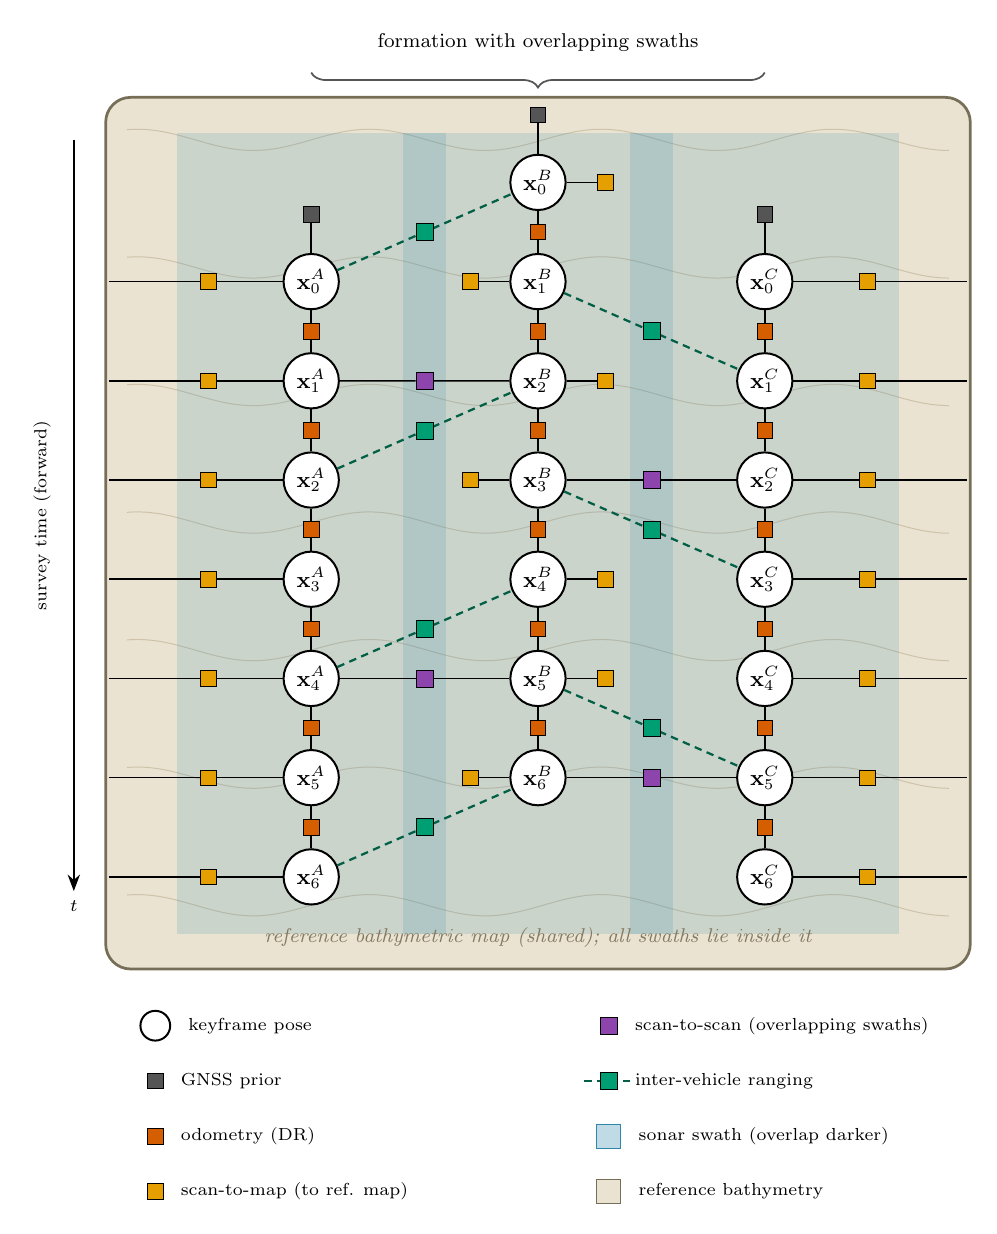
\includegraphics[width=\columnwidth]{figures/formation_factor_graph-1.png}
\caption{Intended TUPER formation graph: shared prior, dead-reckoning, scan-to-map, scan-to-scan, and \mbox{inter-vehicle ranging.}}
\label{fig:formation}
\end{figure}

\textbf{Larger project.} Same WARA-PS stack as \S\ref{sec:cain}. ROSA's managing layer sits above that graph. The managed subsystem is GICP and the OWTT ranging node. The manager holds clock mode, holdover age, ranging dialect, and whether scan-to-map is allowed to pull the team. WASP research supplies the vehicles, the prior map, and the clock. The knowledge is versioned next to the launch files, like the ranging READMEs already are.

\textbf{Adaptation.} Encode those facts as covariances and accept/reject flags the graph already consumes: undisciplined holdover, loosen or drop the OWTT factor; GICP fitness bad, refuse scan-to-map; two-way dead zone, keep one-way. The mapping task continues or aborts with the architecture, which is ROSA's co-adaptation. We currently keep clock mode in firmware and dialect in READMEs. The gap is one tested knowledge model both the graph and an assistant editing a launch file have to satisfy.

\section{Evidence, originality, and GenAI-use transparency}
\label{sec:evidence}

Main sources, by kind:
{\raggedright
\setlength{\leftmargini}{1.1em}
\begin{itemize}
\item Course decks and my June 2026 notes: Feldt L01--L04, Sculley discussion, Frattini requirements slides presented by Robert (Julian did not join), Lenberg guest lecture. \mbox{Course material.}
\item Folkesson WARA-PS TUPER proposal (2024), project proposal.
\item Our paper on TUPER localization and formation. Peer-reviewed, IEEE OCEANS 2025 (Great Lakes). Field protocol that year was TWTT.
\item Our paper on OWTT ranging with a PPS-disciplined OCXO. Accepted at IEEE OCEANS 2026 (Monterey). Ice, harbour, and OCXO holdover. $-48.1$~ppb uncorrected field drift on the three-hour pier moor; $10.8$~cm leftover after 48~h of disciplined free-run. Clear-path harbour RMSE on transmitter~1 is $0.15$~m at the pier and $0.18$~m at the buoy; harbour underway on that transmitter is $3.14$~m.
\item Our paper on bathymetry-aided trajectory correction. Peer-reviewed, IEEE/OES Autonomous Underwater Vehicles Symposium 2026. Pole-mounted vessel with GNSS/INS reference; synthetic drift. Figure~\ref{fig:asko-map} is the overlay from that paper at synthetic $1\%$ of the $1197$~m track. 2D RMSE in that case is $10.46$~m before GICP and $1.62$~m after.
\item \href{https://github.com/smarc-project/smarc2}{\texttt{smarc2}}: CI workflows, contributing README, and LoLo follower-mission README. \mbox{Living software.}
\item Acoustic stack (\href{https://github.com/NinjaTuna007/serial_ping_pkg}{\texttt{serial\_ping\_pkg}}) and serial driver (\href{https://github.com/NinjaTuna007/succorfish_driver}{\texttt{succorfish\_driver}}): tests, configs, per-scenario READMEs, two-way versus one-way split. \mbox{Living software.}
\item K\"{a}stner, CMU \emph{Machine Learning in Production} ch.~1--2 (fetched 2026-09-08 from the public book site). Course book. \mbox{Sole author.}
\item Chowdhury and Cleland-Huang, CAIN 2023. Peer-reviewed full paper. SLR, 15 papers kept. CAIN programs for 2022--2025 contain no underwater paper; this is the closest analog (AI perception on a multi-vehicle uncrewed team).
\item Rezende Silva et al., ROSA, \emph{Frontiers in Robotics and AI}, 2025. Peer-reviewed journal article. Evaluation on the SUAVE AUV \mbox{pipeline-inspection exemplar.}
\end{itemize}}

The project is in our three papers and the WARA-PS proposal. Course decks are the teaching record. The repos, including their READMEs, are the software as it stands. Chowdhury's SLR of 15 papers is indicative of CV-on-sUAS problems. ROSA's SUAVE numbers come from simulation of a single-vehicle mission. The formation graph in \S\ref{sec:rosa} is the intended fleet architecture. No fleet-trial numbers are attached to it.

\textbf{GenAI.} Cursor was used to help research and understand the course concepts, to search for papers, and to help draft. I am responsible for the wording.

\begin{thebibliography}{99}
\raggedright
\sloppy
\bibitem{folkesson}
J.~Folkesson, WARA-PS TUPER proposal, 2024.

\bibitem{oceans2025}
S.~D. Upadhyay et al., TUPER localization and formation, \emph{IEEE OCEANS 2025} (Great Lakes).

\bibitem{oceans2026}
S.~D. Upadhyay et al., OWTT ranging on miniature modems with a PPS-disciplined OCXO, \emph{IEEE OCEANS 2026} \mbox{(Monterey, accepted)}.

\bibitem{auv2026}
S.~D. Upadhyay et al., bathymetry-aided trajectory correction, \emph{IEEE/OES Autonomous Underwater Vehicles Symposium}, 2026.

\bibitem{sculley}
D.~Sculley et al., ``Hidden Technical Debt in Machine Learning Systems,'' \emph{NeurIPS}, 2015.

\bibitem{kastner}
C.~K\"{a}stner, \emph{Machine Learning in Production}, ch.~1--2, MIT Press, 2025, \url{https://mlip-cmu.github.io/book/}.

\bibitem{chowdhury}
M.~T. Chowdhury and J.~Cleland-Huang, ``Engineering Challenges for AI-Supported Computer Vision in Small Uncrewed Aerial Systems,'' \emph{CAIN}, 2023.

\bibitem{rosa}
G.~Rezende Silva et al., ``ROSA: a knowledge-based solution for robot self-adaptation,'' \emph{Frontiers in Robotics and AI}, 2025.

\bibitem{feldt}
R.~Feldt, WASP SE lectures 01--04, June 2026.

\bibitem{frattini}
J.~Frattini, requirements guest-lecture slides, presented by R.~Feldt, 1 June 2026.

\bibitem{lenberg}
P.~Lenberg, BSE guest lecture, 2 June 2026.

\bibitem{smarc2}
\texttt{smarc2}, \url{https://github.com/smarc-project/smarc2}.

\bibitem{acoustic}
Acoustic ranging stack \url{https://github.com/NinjaTuna007/serial_ping_pkg}; serial driver \url{https://github.com/NinjaTuna007/succorfish_driver}.
\end{thebibliography}

\end{document}
